% ****** Start of file apssamp.tex ******
%
%   This file is part of the APS files in the REVTeX 4.2 distribution.
%   Version 4.2a of REVTeX, December 2014
%
%   Copyright (c) 2014 The American Physical Society.
%
%   See the REVTeX 4 README file for restrictions and more information.
%
% TeX'ing this file requires that you have AMS-LaTeX 2.0 installed
% as well as the rest of the prerequisites for REVTeX 4.2
%
% See the REVTeX 4 README file
% It also requires running BibTeX. The commands are as follows:
%
%  1)  latex apssamp.tex
%  2)  bibtex apssamp
%  3)  latex apssamp.tex
%  4)  latex apssamp.tex
%
\documentclass[superscriptaddress,unsortedaddress,
%runinaddress,
%frontmatterverbose, 
%preprint,
%preprintnumbers,
%nofootinbib,
%nobibnotes,
%bibnotes,
 amsmath,amssymb,
 aps,
%pra,
%prb,
%rmp,
%prstab,
%prstper,
%floatfix,
]{revtex4-2}

\usepackage{amsmath}
\usepackage{amsthm}
\usepackage{amssymb}
\usepackage[top=4cm,bottom=4cm,left=2.8cm,right=3.75cm,asymmetric,twoside]{geometry}
\usepackage{graphicx}
\usepackage{fancyhdr}
\usepackage{comment}
\usepackage{tikzorbital}
\usepackage{array} % center tables + 2 next lines
\newcolumntype{P}[1]{>{\centering\arraybackslash}p{#1}}
\newcolumntype{M}[1]{>{\centering\arraybackslash}m{#1}}
\usepackage{multirow} % confusion matrix
\newcommand\MyBox[2]{
  \fbox{\lower0.75cm
    \vbox to 2.0cm{\vfil
      \hbox to 2.0cm{\hfil\parbox{1.4cm}{#1\\#2}\hfil}
      \vfil}%
  }%
}
\usepackage{grffile}
\usepackage{epigraph} % quote
\usepackage{wrapfig} %wrapping text to fig
\usepackage{tikz} %draw figures

\usepackage{subcaption} %subcaption
\usepackage[font=small,labelfont=bf,width=0.9\textwidth]{caption}
\captionsetup[table]{skip=10pt}
\usepackage[T1]{fontenc}
\usepackage[sc, osf]{mathpazo}
\usepackage[euler-digits]{eulervm}
\usepackage{booktabs}
\usepackage{enumerate}
\usepackage{commath}
\usepackage{mathtools}
\usepackage[utf8]{inputenc}
\usepackage{pgfplots}
\usepgfplotslibrary{groupplots,dateplot}
\usetikzlibrary{patterns,shapes.arrows, arrows.meta,bending, shapes,calc,fadings,decorations.pathreplacing,positioning,arrows.meta}
\pgfplotsset{compat=newest}

\usepackage{sansmath}
\tikzset{>=stealth,
OptimumStyle/.style={align=center,anchor=east,rotate=90,font=\scriptsize}
}
\pgfplotsset{%samples=101,
axis lines = left,
every axis plot/.append style={line width=2pt},
}
% Include font for the identity operator
\usepackage{dsfont}
\usepackage[binary-units=true]{siunitx}
\usepackage{makecell}
\usepackage{longtable}
\usepackage{dcolumn}% Align table columns on decimal point
\usepackage{bm}% bold math
\usepackage{physics}
\usepackage{lipsum}
\usepackage{siunitx}
\usepackage{color}
\sisetup{separate-uncertainty}
\pgfplotsset{%samples=101,
axis lines = left,
every axis plot/.append style={line width=2pt},
}

\newcommand{\oliver}[1]{\textcolor{violet}{#1}} 
\newcommand{\morten}[1]{\textcolor{green}{#1}}
\newcommand{\sebastian}[1]{\textcolor{cyan}{#1}}
\newcommand{\marianne}[1]{\textcolor{blue}{#1}}
\newcommand{\oyvind}[1]{\textcolor{maroon}{#1}}
\newcommand{\lasse}[1]{\textcolor{red}{#1}}

\begin{document}

\title{Supplementary Material \\ 
%Predicting Solid State Qubit Candidates}
Predicting Solid State Material Platforms for Quantum Technologies}


\author{Oliver Lerst{\o}l Hebnes}
\affiliation{Department of Physics and Center for Computing in Science Education, University of Oslo, N-0316 Oslo, Norway}
\affiliation{Sopra Steria, N-0185 Oslo, Norway}

\author{Marianne Etzelm\"uller Bathen}
\affiliation{Advanced Power Semiconductor Laboratory, ETH Zürich, 8092  Zürich,  Switzerland}
\affiliation{Department of Physics and Center for Materials Science and Nanotechnology, University of Oslo, N-0316 Oslo, Norway}

\author{{\O}yvind Sigmundson Sch{\o}yen}
\affiliation{Department of Physics and Center for Computing in Science Education, University of Oslo, N-0316 Oslo, Norway}

\author{Sebastian G. Winther-Larsen}
\affiliation{Menon Economics, N-0369 Oslo, Norway}
\affiliation{Department of Physics and Center for Computing in Science Education, University of Oslo, N-0316 Oslo, Norway}

\author{Lasse Vines}
\affiliation{Department of Physics and Center for Materials Science and Nanotechnology, University of Oslo, N-0316 Oslo, Norway}

\author{Morten Hjorth-Jensen}
\affiliation{Department of Physics and Astronomy and Facility for Rare Ion Beams, Michigan State University, East Lansing, MI 48824, USA}
\affiliation{Department of Physics and Center for Computing in Science Education, University of Oslo, N-0316 Oslo, Norway}

\pacs{02.70.Ss, 31.15.A-, 31.15.bw, 71.15.-m, 73.21.La}

\maketitle


Contents: \\ 
Supplementary methods --- additional information on the featurization process and implementation of the machine learning models. \\ 
Supplementary results --- tables over the materials that were predicted by the machine learning models based on the training sets derived using the three different data mining approaches. \\ 
Supplementary references. 


\newpage 

\section*{Supplementary methods}
\subsection*{Featurization}
Table~\ref{table:featurizers} contains an overview of this work's chosen 39 features from matminer. The features were selected based on
the work of 


\begin{center}
\begin{longtable}{M{3.5cm} M{6.5cm} M{2.0cm}}
\caption{This work's chosen 39 featurizers from Matminer. Descriptions are either found from Ref. \cite{Ward2018} or from the project's Github page. For entries lacking references, we refer to Ref.~\cite{Ward2018}.}
\label{table:featurizers} 
\\ \hline
Features & Description & Reference \\
\hline 
  \textbf{Composition features} & & \\ 
  AtomicOrbitals & Highest occupied molecular orbital (HOMO) & \cite{Kotochigova1997}  \\   
   & and lowest unoccupied molecular orbital (LUMO) &  \\   
  AtomicPacking-Efficiency & Packing efficiency & \cite{Laws2015}  \\   
  BandCenter & Estimate absolute position of band center  & \cite{Butler1978} \\   
   & using geometric mean of electronegativity &  \\  
  ElementFraction & Fraction of each element in a composition &    \\   
  ElementProperty & Statistics of various element properties & \cite{Ong2013,Ward2016, Deml2016}  \\   
  IonProperty & Maximum and average ionic character & \cite{Ward2016} \\   
  Miedema & Formation enthalpies of intermetallic compounds, solid solutions, & \cite{Weeber1987} \\   
   & and amorphous phases using semi-empirical Miedema model &  \\   
  Stoichiometry & $L^p$ norm-based stoichiometric attributes & \cite{Ward2016} \\   
  TMetalFraction & Fraction of magnetic transition metals & \cite{Deml2016}  \\   
  ValenceOrbital & Valence orbital attributes such as & \cite{Ward2016}  \\   
   &  the mean number of electrons in each shell &   \\   
  YangSolid-Solution & Mixing thermochemistry and size mismatch terms & \cite{Yang2012} \\
    \hline 
  \textbf{Oxide composition features} &  &  \\
  Electronegativity-Diff & Statistics on electronegativity difference & \cite{Deml2016} \\   
   &  between anions and cations & \\ 
  OxidationStates & Statistics of oxidation states & \cite{Deml2016}  \\   
\hline 
  \textbf{Structure features} & & \\   
  DensityFeatures & Calculate density, volume per atom and packing fraction & - \\   
  GlobalSymmetry-Features & Determines spacegroup number, crystal system  & - \\   
   & (1-7) and inversion symmetry & \\ 
  RadialDistribution-Function & Calculates the radial distribution  & - \\   
   & function of a crystal system & \\ 
  CoulombMatrix & Generate the Coulomb matrix for nuclear interactions  & \cite{Rupp2012}  \\    
  %CoulombMatrix & Generate the Coulomb matrix, which is a representation of the nuclear coulombic interaction of the input structure. & \cite{Rupp2012}  \\      
  PartialRadial-Distribution-Function & Compute the partial radial distribution  & \cite{Schuett2014}  \\   
   & function of a crystal structure & \\ 
  SineCoulomb-Matrix & Computes a variant of the coulomb matrix & \cite{Faber2015}  \\   
   & developed for periodic crystals & \\ 
  EwaldEnergy & Computes the energy from Coulombic interactions  & \cite{Ewald1921}  \\   
   & based on charge states of each site & \\ 
  BondFractions & Compute the fraction of each bond in a  & \cite{Hansen2015}  \\   
   & structure, based on nearest neighbors & \\ 
  Structural Heterogeneity & Calculates the variance in bond lengths and  & \cite{Ward2017}  \\   
   & atomic volumes in a structure & \\ 
  MaximumPacking-Efficiency & Calculates the maximum packing efficiency of a structure & \cite{Ward2017} \\   
  Chemical-Ordering & Computes how much the ordering of species  & \cite{Ward2017}  \\   
   & differs from random in a structure & \\ 
  XRDPowder-Pattern & 1D array representing normalized powder diffraction & \cite{Ong2013} \\ 
   &of a structure as calculated by pymatgen  & \\ 
    \hline 
  \textbf{Site features} & & \\
  AGNI-Fingerprints & Calculates the product integral of RDF & \cite{Botu2014}  \\    
   & and Gaussian window function  & \\ 
  AverageBond- Agle & Determines the average bond angle of a specific  & \cite{Jong2016}  \\
   & site with its nearest neighbors  & \\ 
  AverageBond-Length & Determines the average bond length between one specific site & \cite{Jong2016}  \\ 
   & and all its nearest neighbors  & \\ 
  BondOrientational-Parameter & Calculates the averages of spherical  & \cite{Seko2017, Steinhardt1983}  \\ 
   & harmonics of local neighbors & \\ 
  ChemEnvSite-Fingerprint & Calculates the resemblance of given sites to ideal & \cite{Waroquiers2017, Zimmermann2017}  \\   
   & environment using pymatgens ChemEnv package  & \\ 
  Coordination-Number & The number of first nearest neighbors of a site & \cite{Zimmermann2017}  \\
  CrystalNN-Fingerprint & A local order parameter fingerprint for periodic crystals & -  \\   
  GaussianSymm-Func & Calculates the gaussian radial and angular symmetry functions  & \cite{Behler2011,Khorshidi2016}  \\   
   & originally suggested for fitting machine learning potentials &  \\ 
  GeneralizedRadial-Distribution-Function & Computes the general radial distribution function for a site & \cite{Seko2017}  \\   
  LocalProperty-Difference & Computes the difference in elemental properties  & \cite{Ward2017, Jong2016} \\   
   & between a site and its neighboring sites & \\ 
  OPSite-Fingerprint & Computes the local structure order parameters & \cite{Zimmermann2017} \\   
   & from a site's neighbor environment  & \\ 
  Voronoi-Fingerprint & Calculates the Voronoi tessellation-based  & \cite{Peng2011,Wang2019} \\
   & features around a target site & \\ 
\hline     
  \textbf{Density of state features} & & \\
  DOSFeaturizer & Computes top contributors to the density of  & \cite{Dylla2020} \\ 
  & states at the VBM and CBM  & \\ 
  %DOSFeaturizer & Computes top contributors to the density of states at the valence and conduction band edges. Thus includes chemical species, orbital character, and orbital location information. & \cite{Dylla2020} \\
  \hline  
  \textbf{Band structure features} & & \\
  BandFeaturizer & Converts a complex electronic band  & - \\ 
   &structure into discrete quantities  & \\ 
%BandFeaturizer & Converts a complex electronic band structure into quantities such as band gap and the norm of k point coordinates at which the conduction band minimum and valence band maximum occur. & - \\
\hline 
\end{longtable}
\end{center}


\subsection*{Optimization of machine learning models}

In the evaluation of the approaches, we apply a $5\times 5$ stratified cross-validation when searching for the optimal hyperparameter combinations. Four different evaluation metrics are applied to each of the four algorithms for each approach. 

For random forest, gradient boost, and decision tree, we found that by adjusting most of the available parameters responded to severe overfitting. Therefore, most parameters are the default values defined by Scikit-learn. The only parameter that we found that could potentially improve the evaluation metric F$1$ was the maximum number of depth for the trees grown, which we adjusted between $1$ and $8$. For logistic regression, we chose to adjust the regularization strength with seven logarithmic adjusted values from $10^{-3}$ to $10^{5}$, and use either $200$ or $400$ iterations to reach convergence. 

When searching for the optimal number of principal components, we iterated over every odd number of principal components from $1$ to the upper restricted number which defines an accumulated variance of $95 \ \%$ from the principal component analysis. Due to a large number of principal components, we end up fitting $25$ folds for each of the $1232$ parameter combinations, totaling up to $30.800$ individual models, just for logistic regression for one approach.

%Ferrenti 
We visualize the grid search for the optimal number of principal components for the Ferrenti approach in Figure~\ref{fig:01-pca}, where we present the mean accuracy on the training set, and the balanced accuracy, precision, recall, and F$1$-score on the test set as a function of principal components used in the models. For each principal component, the optimal combination of hyperparameters based on the F$1$-score is visualized. 

In Table~\ref{tab:01-pc}, we find the precise measurements for each of the evaluation metrics for the optimal number of principal components, which is visualized as dotted lines in Fig.~\ref{fig:01-pca}. The relevant hyperparameters for logistic regression were the maximum iterations, which was set at $400$, and the regularization term, which was found optimal at $0.46$. For random forest and decision trees, we find the maximum depth of $7$, while being $4$ for gradient boost. We find the best performing model is logistic regression, but is dependent on a large amount of principal components. 

%Augmented ferrenti (to be continued)
%Intuitive (to be continued)

\begin{table}[!ht]
\centering
\caption{A table of the optimal number of principal components and the respective scores (standard deviation) for the Ferrenti approach, as visualized in the dash-dotted line in figure \ref{fig:01-pca}.}
\label{tab:01-pc}
\noindent\makebox[\textwidth]{
\begin{tabular}{M{1.0cm} M{1.0cm} M{2.0cm} M{2.0cm}M{2.0cm}M{2.0cm} }
  \hline
  \hline
   Model & PC & Mean test &  Mean precision & Mean recall & mean F1\\
  \hline
  LOG & $171$ & $0.98(0.012)$ & $0.98(0.011)$ & $0.99(0.007)$ & $0.99(0.007)$ \\
  DT & $37$   & $0.77(0.034)$ & $0.84(0.034)$ & $0.85(0.044)$ & $0.84(0.022)$ \\
  RF & $53$   & $0.87(0.027)$ & $0.88(0.022)$ & $0.98(0.010)$ & $0.93(0.014)$ \\
  GB & $107$  & $0.92(0.016)$ & $0.92(0.015)$ & $0.98(0.010)$ & $0.95(0.009)$ \\
  \hline
\end{tabular}
}
\end{table}


\begin{figure}[ht!]
\begin{subfigure}[b]{1.0\textwidth}
    \centering
    % This file was created by tikzplotlib v0.9.8.
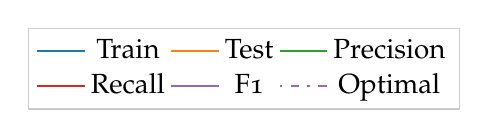
\begin{tikzpicture}

\definecolor{color0}{rgb}{0.12156862745098,0.466666666666667,0.705882352941177}
\definecolor{color1}{rgb}{1,0.498039215686275,0.0549019607843137}
\definecolor{color2}{rgb}{0.172549019607843,0.627450980392157,0.172549019607843}
\definecolor{color3}{rgb}{0.83921568627451,0.152941176470588,0.156862745098039}
\definecolor{color4}{rgb}{0.580392156862745,0.403921568627451,0.741176470588235}
\begin{axis}[%
 hide axis,
 xmin=10,
 xmax=50,
 ymin=0,
 ymax=0.4,
 legend columns=3,
 legend style={
   fill opacity=1,
   draw opacity=1,
   text opacity=1,
   align=center,
   anchor=north,
   draw=white!80!black
 },
 ]
 \addlegendimage{semithick, color0}
 \addlegendentry{Train};
 \addlegendimage{semithick, color1}
 \addlegendentry{Test};
 \addlegendimage{semithick, color2}
 \addlegendentry{Precision};
 \addlegendimage{semithick, color3}
 \addlegendentry{Recall};
 \addlegendimage{semithick, color4}
 \addlegendentry{F1};
 \addlegendimage{semithick, color4, dash pattern=on 1pt off 3pt on 3pt off 3pt}
 \addlegendentry{Optimal};
 \end{axis}

\end{tikzpicture}

  \end{subfigure}
  \par\bigskip
  \begin{subfigure}[b]{0.5\textwidth}
    % This file was created by tikzplotlib v0.9.8.
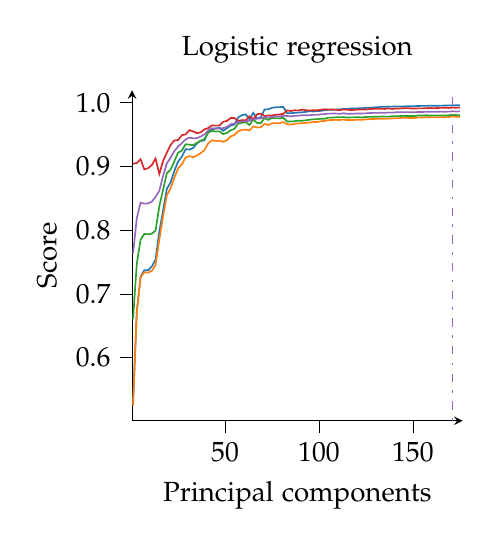
\begin{tikzpicture}

\definecolor{color0}{rgb}{0.12156862745098,0.466666666666667,0.705882352941177}
\definecolor{color1}{rgb}{1,0.498039215686275,0.0549019607843137}
\definecolor{color2}{rgb}{0.172549019607843,0.627450980392157,0.172549019607843}
\definecolor{color3}{rgb}{0.83921568627451,0.152941176470588,0.156862745098039}
\definecolor{color4}{rgb}{0.580392156862745,0.403921568627451,0.741176470588235}

\begin{axis}[
height=2.275590092707901in,
tick align=outside,
tick pos=left,
title={Logistic regression},
width=2.275590092707901in,
x grid style={white!69.0196078431373!black},
xlabel={Principal components},
xmin=0.5, xmax=176.5,
xtick style={color=black},
xtick={0,50,100,150,200},
xticklabels={
  \(\displaystyle {0}\),
  \(\displaystyle {50}\),
  \(\displaystyle {100}\),
  \(\displaystyle {150}\),
  \(\displaystyle {200}\)
},
y grid style={white!69.0196078431373!black},
ylabel={Score},
ymin=0.501096391747291, ymax=1.01973669481458,
ytick style={color=black},
ytick={0.5,0.6,0.7,0.8,0.9,1,1.1},
yticklabels={
  \(\displaystyle {0.5}\),
  \(\displaystyle {0.6}\),
  \(\displaystyle {0.7}\),
  \(\displaystyle {0.8}\),
  \(\displaystyle {0.9}\),
  \(\displaystyle {1.0}\),
  \(\displaystyle {1.1}\)
}
]
\addplot [semithick, color0]
table {%
1 0.527978311919052
3 0.672257518373159
5 0.726936676480703
7 0.737204003963955
9 0.7371536474315
11 0.743129561041308
13 0.753973065365214
15 0.797999916812017
17 0.831220812266941
19 0.864665747038822
21 0.875225642897371
23 0.892940839297993
25 0.907831289942227
27 0.915484280258436
29 0.927154832624676
31 0.926581906722074
33 0.929048501041305
35 0.936214158404711
37 0.940204028671267
39 0.940954212283905
41 0.954348432567421
43 0.9579101829613
45 0.95979102944338
47 0.960507784158689
49 0.95611045233101
51 0.959989942496352
53 0.964312267547714
55 0.965762937077656
57 0.977118861393655
59 0.980625775462163
61 0.981674131523199
63 0.973849068329029
65 0.98417222600597
67 0.975393355577146
69 0.976988296303105
71 0.98932929153175
73 0.989743808970333
75 0.992040327743967
77 0.992880248748514
79 0.993137411653601
81 0.993414113504208
83 0.983692753729346
85 0.983623389884701
87 0.984284121882561
89 0.98452486392549
91 0.985083047934706
93 0.98566681374314
95 0.98664953042687
97 0.986322636640174
99 0.986746837221478
101 0.987259146957983
103 0.988267587421691
105 0.98885404647408
107 0.989065862475352
109 0.989253542413724
111 0.989730781585175
113 0.990150137134204
115 0.990077108383256
117 0.991006827686701
119 0.991019162207793
121 0.991312771079592
123 0.991361059142255
125 0.992209056565552
127 0.991993392467355
129 0.992711089064495
131 0.992935244750097
133 0.993596095870027
135 0.993493678432798
137 0.993889977274
139 0.993922059204236
141 0.994264579115255
143 0.994260783657537
145 0.994219836836825
147 0.994575058305901
149 0.994623827364361
151 0.994689063658078
153 0.99491757821692
155 0.995104843642357
157 0.995059970812512
159 0.995513002930682
161 0.995309109938055
163 0.995398594494915
165 0.99546426365274
167 0.995623313596039
169 0.995868153409378
171 0.995729627261883
173 0.996162135584249
175 0.995978665616529
};
\addplot [semithick, color1]
table {%
1 0.524670950977623
3 0.670867772619925
5 0.725863108394313
7 0.733927442763526
9 0.733555795752711
11 0.736184000561332
13 0.745465701046404
15 0.785273990017892
17 0.821643763767867
19 0.854757534127692
21 0.865826097874878
23 0.882614449866961
25 0.896823087639802
27 0.903405199983751
29 0.914149433405531
31 0.916217593233734
33 0.914707877943531
35 0.917110720886905
37 0.92093593844921
39 0.925600873572896
41 0.936269081594404
43 0.941212773441611
45 0.940024320077405
47 0.940302539473271
49 0.938740125450312
51 0.94121085355698
53 0.947146572274262
55 0.949563968303208
57 0.955407434232757
59 0.957350491811754
61 0.957949057276174
63 0.956670804181923
65 0.962797141730786
67 0.961288712057005
69 0.961339015896405
71 0.966930102166114
73 0.965076521181973
75 0.967955056050106
77 0.967817135951282
79 0.968013692622731
81 0.969581622101708
83 0.966388905661144
85 0.965800496335647
87 0.966843609493896
89 0.967544083948675
91 0.968048265317993
93 0.968286007415491
95 0.968979568623758
97 0.969720057370344
99 0.969798328560165
101 0.97100459313587
103 0.971399663293135
105 0.972718471238199
107 0.972996212393989
109 0.973160320291597
111 0.972949300089185
113 0.973716280843254
115 0.972803655674531
117 0.972867637364768
119 0.973066455059281
121 0.973436930935855
123 0.973276997021617
125 0.973800030559356
127 0.974367715378834
129 0.974564924321739
131 0.974746235013452
133 0.975019149914415
135 0.974825636714805
137 0.975136478915891
139 0.975366177255345
141 0.975933383834747
143 0.97593290559467
145 0.976490474897936
147 0.976224936250044
149 0.97611034651171
151 0.976116303278068
153 0.977110417139829
155 0.976754404794218
157 0.977391375798836
159 0.977141909433516
161 0.977032624190085
163 0.977401491315049
165 0.977503878545485
167 0.977239470409126
169 0.977584888998447
171 0.978416503714208
173 0.977958582378238
175 0.978155313081066
};
\addplot [semithick, color2]
table {%
1 0.660526209531335
3 0.747271763749716
5 0.784917402501545
7 0.794267176756586
9 0.793511475403584
11 0.794620562078218
13 0.799523152230156
15 0.837581215874355
17 0.863697781589945
19 0.889480285672649
21 0.895088519217677
23 0.908204106634087
25 0.921655479971229
27 0.924944626117226
29 0.934982733626013
31 0.934221489453499
33 0.933492384550335
35 0.937090811707038
37 0.940412513912378
39 0.942984820378985
41 0.953053634341826
43 0.955921520338845
45 0.954978817159891
47 0.955164046043096
49 0.950861081645013
51 0.952776616955171
53 0.956619619067437
55 0.959181649945466
57 0.967304721177759
59 0.968682184215419
61 0.969544860690647
63 0.965172494479605
65 0.973618553063717
67 0.968434814374178
69 0.967925791547072
71 0.975634040039191
73 0.973176998920976
75 0.97621418482231
77 0.975489402808498
79 0.9754573020742
81 0.976602372231858
83 0.970652590698134
85 0.970663060426771
87 0.971014489855003
89 0.971919589679479
91 0.971795111996232
93 0.972508187686635
95 0.973404234589117
97 0.97400655763931
99 0.974200947121328
101 0.97495293560689
103 0.974922176310523
105 0.976618141603626
107 0.976796274124154
109 0.977163964798968
111 0.977310022601592
113 0.977527482926915
115 0.976778742617798
117 0.977109804939133
119 0.977138645750667
121 0.977317819037685
123 0.976950737393212
125 0.977715629784876
127 0.977895865047589
129 0.977924905340252
131 0.978112332680922
133 0.978327531824792
135 0.978320150536469
137 0.978162442434481
139 0.97887430522476
141 0.979094557757062
143 0.979083321261843
145 0.979465600334943
147 0.979096858028989
149 0.979273497447592
151 0.979264647632088
153 0.98019568430901
155 0.979852563049805
157 0.980407553452011
159 0.97987666478631
161 0.980033763597739
163 0.980239959065847
165 0.980222596059216
167 0.979858928781099
169 0.980414030151713
171 0.98099643138722
173 0.98060989765861
175 0.980626337513261
};
\addplot [semithick, color3]
table {%
1 0.904293639406982
3 0.905471066475371
5 0.911330463892874
7 0.895509325681492
9 0.89726924916308
11 0.902149210903874
13 0.912498326159732
15 0.888276422764228
17 0.908609277857484
19 0.921690100430416
21 0.933788617886179
23 0.940827355332377
25 0.94160306073649
27 0.949027259684362
29 0.950390243902439
31 0.95703299856528
33 0.955081779053085
35 0.952342419894787
37 0.953516021042563
39 0.958209469153515
41 0.960153993304639
43 0.9646456241033
45 0.964064084170254
47 0.964260162601626
49 0.970118603538976
51 0.971485413677666
53 0.976172166427547
55 0.97597800095648
57 0.971487326637972
59 0.972854136776662
61 0.972268770923003
63 0.978711621233859
65 0.974419894787183
67 0.981837398373984
69 0.983006217120995
71 0.979104734576758
73 0.980082257293161
75 0.980083213773314
77 0.981252032520325
79 0.981645145863223
81 0.982618842659015
83 0.988089909134386
85 0.986916307986609
87 0.988285031085605
89 0.987893830703013
91 0.989262553802009
93 0.988286944045911
95 0.987894787183166
97 0.988285031085605
99 0.988090865614539
101 0.989068388330942
103 0.98984887613582
105 0.989262553802009
107 0.989457675753228
109 0.989068388330942
111 0.988285987565758
113 0.989459588713534
115 0.989069344811095
117 0.988483022477284
119 0.988874222859876
121 0.989264466762315
123 0.989655667144907
125 0.989263510282162
127 0.990044954567193
129 0.990436154949785
131 0.990435198469632
133 0.990630320420851
135 0.990240076518412
137 0.99121568627451
139 0.990240076518412
141 0.99102056432329
143 0.991019607843137
145 0.991410808225729
147 0.991606886657102
149 0.99102056432329
151 0.991019607843137
153 0.99121568627451
155 0.991214729794357
157 0.991410808225729
159 0.991996174079388
161 0.991410808225729
163 0.991801052128168
165 0.991996174079388
167 0.992191296030607
169 0.991801052128168
171 0.992386417981827
173 0.992191296030608
175 0.992581539933046
};
\addplot [semithick, color4]
table {%
1 0.76327826913597
3 0.818651569656171
5 0.843331146676396
7 0.84169792475628
9 0.842067908612409
11 0.844813503673515
13 0.852124363378905
15 0.861976720922363
17 0.885282648968169
19 0.90496551535333
21 0.913808723923361
23 0.924073146040379
25 0.931375978080348
27 0.936731426464567
29 0.942533198420864
31 0.945370642159646
33 0.944072143424975
35 0.944579525921237
37 0.946839897656345
39 0.950460462558033
41 0.956470634227884
43 0.960164381825251
45 0.959398895015101
47 0.959577982179569
49 0.960312496475416
51 0.961950228479052
53 0.966214111548991
55 0.967423688855172
57 0.969320345634248
59 0.970697341062533
61 0.970854625027329
63 0.971833175254563
65 0.973959307480675
67 0.975027042687256
69 0.975346597911891
71 0.977319633868194
73 0.97657707431891
75 0.978095920537375
77 0.978319877721788
79 0.978511612913037
81 0.979567956211785
83 0.979238141098257
85 0.978651945000747
87 0.979519430282232
89 0.979793635143959
91 0.980395644616177
93 0.9802832228004
95 0.980553741070374
97 0.981048727805319
99 0.981042530303693
101 0.981911935989541
103 0.98229786639816
105 0.982860073758902
107 0.983051506088867
109 0.983041644918783
111 0.982736151995381
113 0.983428784105583
115 0.982852244274254
117 0.982737730874411
119 0.982936953339814
121 0.983228597277582
123 0.983234206366182
125 0.983421162390887
127 0.98390753416485
129 0.984105263945853
131 0.984201711076164
133 0.984398525513513
135 0.984201523780763
137 0.984602971088457
139 0.984486514671602
141 0.984981991879854
143 0.984983090467204
145 0.985365284099043
147 0.985277860703882
149 0.98507709601412
151 0.985075740767988
153 0.985643232324871
155 0.985463068376293
157 0.985842563116465
159 0.98585600923236
161 0.985655424765855
163 0.985952037646302
165 0.986039552285513
167 0.985952994477143
169 0.986040974394843
171 0.986623508036311
173 0.986333887205196
175 0.986530816878293
};
\addplot [semithick, color4, dash pattern=on 1pt off 3pt on 3pt off 3pt]
table {%
171 0.501096391747291
171 1.01973669481458
};
\end{axis}

\end{tikzpicture}

    \caption{}
    \label{fig:q1-LOG}
  \end{subfigure}%
    \hfill
  \begin{subfigure}[b]{0.5\textwidth}
    % This file was created by tikzplotlib v0.9.8.
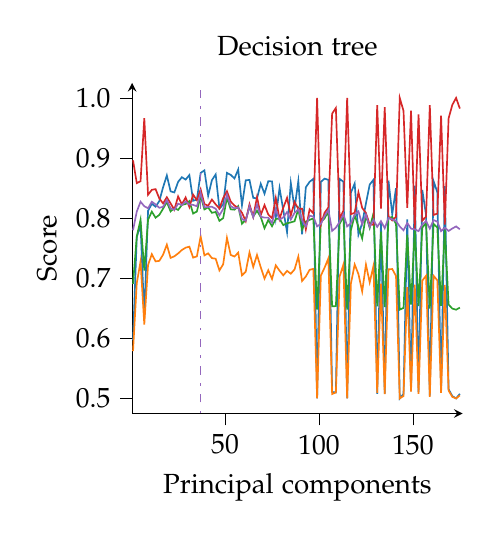
\begin{tikzpicture}

\definecolor{color0}{rgb}{0.12156862745098,0.466666666666667,0.705882352941177}
\definecolor{color1}{rgb}{1,0.498039215686275,0.0549019607843137}
\definecolor{color2}{rgb}{0.172549019607843,0.627450980392157,0.172549019607843}
\definecolor{color3}{rgb}{0.83921568627451,0.152941176470588,0.156862745098039}
\definecolor{color4}{rgb}{0.580392156862745,0.403921568627451,0.741176470588235}

\begin{axis}[
height=2.275590092707901in,
tick align=outside,
tick pos=left,
title={Decision tree},
width=2.275590092707901in,
x grid style={white!69.0196078431373!black},
xlabel={Principal components},
xmin=0.5, xmax=176.5,
xtick style={color=black},
xtick={0,50,100,150,200},
xticklabels={
  \(\displaystyle {0}\),
  \(\displaystyle {50}\),
  \(\displaystyle {100}\),
  \(\displaystyle {150}\),
  \(\displaystyle {200}\)
},
y grid style={white!69.0196078431373!black},
ylabel={Score},
ymin=0.475, ymax=1.025,
ytick style={color=black},
ytick={0.4,0.5,0.6,0.7,0.8,0.9,1,1.1},
yticklabels={
  \(\displaystyle {0.4}\),
  \(\displaystyle {0.5}\),
  \(\displaystyle {0.6}\),
  \(\displaystyle {0.7}\),
  \(\displaystyle {0.8}\),
  \(\displaystyle {0.9}\),
  \(\displaystyle {1.0}\),
  \(\displaystyle {1.1}\)
}
]
\addplot [semithick, color0]
table {%
1 0.596497717449444
3 0.768506780224986
5 0.789072473394637
7 0.635431052744238
9 0.812246594635627
11 0.823822913593586
13 0.819063114844103
15 0.828455297352151
17 0.851312841778874
19 0.871054460654502
21 0.844573082460765
23 0.842712085180569
25 0.860318528354227
27 0.868077782369472
29 0.864111971448012
31 0.871685010557694
33 0.828865734907841
35 0.830932878731714
37 0.875222132631586
39 0.879464758724772
41 0.837337279686309
43 0.863188141109501
45 0.872661827996532
47 0.815872474339355
49 0.822693179431544
51 0.875248923103878
53 0.87197968309829
55 0.865976578541978
57 0.880933944970876
59 0.821406402368332
61 0.862939330364918
63 0.863531425331119
65 0.833696454122586
67 0.83298007274486
69 0.857111340325214
71 0.840624043555583
73 0.861380554172503
75 0.861108374817675
77 0.800606474192092
79 0.850138667208445
81 0.813133334410096
83 0.776733277842867
85 0.858524949760363
87 0.816409811034941
89 0.861656021029682
91 0.772931198434995
93 0.851300184110581
95 0.860396061377324
97 0.865314146220163
99 0.5
101 0.860272513457213
103 0.865730323533595
105 0.863562280432173
107 0.510780648950084
109 0.510025077065436
111 0.865172729428312
113 0.860575017255092
115 0.5
117 0.842407371293759
119 0.85746071020843
121 0.772354167423015
123 0.791509904415402
125 0.824349545979451
127 0.855896205345502
129 0.863750622916912
131 0.507692855226488
133 0.794366735038516
135 0.507977055241831
137 0.86246681579223
139 0.80625641462588
141 0.849912698261898
143 0.5
145 0.507400252960791
147 0.797810076370395
149 0.512379354442437
151 0.854027328023614
153 0.510660948072043
155 0.846926636549466
157 0.805216696040322
159 0.504692860701829
161 0.861615559155597
163 0.843237281200769
165 0.51268667018346
167 0.853159400642768
169 0.515295944317397
171 0.503806676631789
173 0.5
175 0.507660067968993
};
\addplot [semithick, color1]
table {%
1 0.578768326842932
3 0.691790567314599
5 0.727748869488468
7 0.623064681508728
9 0.721959461305946
11 0.740025114989964
13 0.728012304526293
15 0.728950643408319
17 0.739168797050791
19 0.755813493294483
21 0.733819262180812
23 0.736502631243664
25 0.74123106381643
27 0.746944824666848
29 0.750800204129114
31 0.752515759303062
33 0.734273446227535
35 0.736303831552397
37 0.769742552657187
39 0.738027412942765
41 0.741400498828404
43 0.73342747646191
45 0.732457103803948
47 0.712984303015867
49 0.723216204214052
51 0.767099409308878
53 0.738716267917846
55 0.736103655305234
57 0.742504820715366
59 0.704777293844367
61 0.710847611292375
63 0.742733149884872
65 0.718701609120906
67 0.738685802732431
69 0.718188129767398
71 0.69930786751088
73 0.713248353395412
75 0.698764008833593
77 0.721435647627542
79 0.712593752135
81 0.704805617566737
83 0.712219320622118
85 0.707513599836771
87 0.714646026637418
89 0.736076347150594
91 0.695413534563463
93 0.702911964588077
95 0.713967476905067
97 0.715624707562656
99 0.5
101 0.704367860789669
103 0.717735700344739
105 0.733097151978788
107 0.507334628643811
109 0.509988134475939
111 0.702994975247845
113 0.722606732937077
115 0.5
117 0.69098720892444
119 0.722855625045008
121 0.70701382280005
123 0.677964524834324
125 0.72265892988705
127 0.693069657328983
129 0.720387790383128
131 0.50918391562294
133 0.690996190236147
135 0.507213854098
137 0.714920114980732
139 0.715284894445583
141 0.703893530187289
143 0.5
145 0.504043067457702
147 0.685176994067238
149 0.511407359450042
151 0.689459213415096
153 0.507687988511159
155 0.696004412180165
157 0.704069485605712
159 0.502599868160844
161 0.704102806382936
163 0.696546110006297
165 0.509182134686439
167 0.6889112523058
169 0.51316191934915
171 0.502532190727313
173 0.5
175 0.505121743489749
};
\addplot [semithick, color2]
table {%
1 0.690646028080078
3 0.76977795012896
5 0.797266579935977
7 0.712665710384953
9 0.797395011924239
11 0.810835730414563
13 0.800721666817829
15 0.805359862993895
17 0.815671846991249
19 0.826815874616206
21 0.811172521251474
23 0.816976708496276
25 0.81355840819195
27 0.822062539826173
29 0.823422923735299
31 0.828356808638562
33 0.807611589533691
35 0.811008393709643
37 0.836904435636554
39 0.814477964339968
41 0.817791500401826
43 0.808810170628359
45 0.810276907853969
47 0.795481007683356
49 0.800014895188039
51 0.833907288587748
53 0.814636312882636
55 0.8140703790893
57 0.820045019066581
59 0.790604112329787
61 0.797295667094074
63 0.81881134153839
65 0.802738911050435
67 0.812316041527201
69 0.801834690970316
71 0.783252195964148
73 0.796868551574173
75 0.786516502608262
77 0.798731034138699
79 0.798962968289488
81 0.788423442064658
83 0.791442017252198
85 0.792905154664528
87 0.794769766926958
89 0.814926677788018
91 0.7812266796863
93 0.794165600658011
95 0.79717622519109
97 0.799454716161802
99 0.647691969811924
101 0.793185246483871
103 0.799651045331469
105 0.811755230940412
107 0.653249710619967
109 0.653576827149121
111 0.79003483898687
113 0.80343891381361
115 0.647691969811924
117 0.77975373251055
119 0.804913195581554
121 0.785309784717675
123 0.766122974132401
125 0.804872282827964
127 0.783694457722852
129 0.80752545515596
131 0.653152567864102
133 0.777494620076289
135 0.652107381621955
137 0.80007840746219
139 0.802023435566857
141 0.790203831225899
143 0.647691969811924
145 0.650558738663497
147 0.772575263592028
149 0.656266076861863
151 0.782563328714032
153 0.653630757156716
155 0.78415133429832
157 0.791886530924938
159 0.649509593014578
161 0.79044713997428
163 0.784492867064612
165 0.654206818351503
167 0.781295695131415
169 0.656166518971361
171 0.649420327841799
173 0.647691969811924
175 0.651030218400474
};
\addplot [semithick, color3]
table {%
1 0.896108082257293
3 0.85820468675275
5 0.861334289813486
7 0.96641893830703
9 0.838841702534672
11 0.847083692013391
13 0.848228598756576
15 0.832624581539933
17 0.824447632711621
19 0.834783357245337
21 0.8244725011956
23 0.814092778574845
25 0.836130081300813
27 0.822876135820182
29 0.834383548541368
31 0.81838737446198
33 0.839061692969871
35 0.829908177905309
37 0.847869918699187
39 0.823249163079866
41 0.820719273075084
43 0.830870396939264
45 0.822864658058345
47 0.816020086083214
49 0.833195600191296
51 0.844739359158298
53 0.827567670970827
55 0.820901004304161
57 0.816808225729316
59 0.808959349593496
61 0.795131516021043
63 0.823043519846963
65 0.802168340506935
67 0.834984218077475
69 0.805073170731707
71 0.821659493065519
73 0.806078431372549
75 0.799786704925873
77 0.833614538498326
79 0.798639885222382
81 0.817378287900526
83 0.833779053084649
85 0.804682926829268
87 0.826782400765184
89 0.815418460066954
91 0.815595408895265
93 0.781271162123386
95 0.814672405547585
97 0.808028694404591
99 1
101 0.789662362505978
103 0.808978479196557
105 0.817758010521282
107 0.973787661406026
109 0.983219512195122
111 0.79885031085605
113 0.812475370636059
115 1
117 0.806649450023912
119 0.808787183165949
121 0.842985174557628
123 0.817000478240077
125 0.808599713055954
127 0.789263510282162
129 0.789034911525586
131 0.98809756097561
133 0.816023912003826
135 0.984585365853659
137 0.802546150167384
139 0.796284074605452
141 0.802133907221425
143 1
145 0.978536585365854
147 0.816975609756098
149 0.978731707317073
151 0.781843137254902
153 0.972682926829268
155 0.79591487326638
157 0.802318507890961
159 0.98790243902439
161 0.805261597321856
163 0.80745193687231
165 0.970275466284074
167 0.789251076040172
169 0.965982783357245
171 0.988487804878049
173 1
175 0.982219033955045
};
\addplot [semithick, color4]
table {%
1 0.779835815655286
3 0.810860357787374
5 0.827212136873701
7 0.819854736749766
9 0.816362260142288
11 0.827301018796805
13 0.822822811449125
15 0.817161204645316
17 0.818798213116716
19 0.830143105303606
21 0.816410276017348
23 0.813713650026485
25 0.824109298073981
27 0.821822540679694
29 0.827699790006685
31 0.822652858207086
33 0.822008073434729
35 0.81974863919911
37 0.841067190862751
39 0.817987020508943
41 0.818622639639426
43 0.818890811753971
45 0.81559144725181
47 0.804581546338155
49 0.815380439624153
51 0.838892195269103
53 0.819884850253967
55 0.816329074489787
57 0.81783619879634
59 0.798561424747511
61 0.795564081309575
63 0.819974877318493
65 0.801543267470842
67 0.822747956329741
69 0.802453099769105
71 0.800780858809059
73 0.800860868596634
75 0.792196807552761
77 0.814402840887597
79 0.797347626490337
81 0.801355119305887
83 0.810126352140618
85 0.797672935774432
87 0.808814427555639
89 0.81448538251746
91 0.796528005130148
93 0.786050925371033
95 0.804089631659403
97 0.802547088574708
99 0.786180105478537
101 0.790386746819531
103 0.803759748113057
105 0.813563395829392
107 0.778803831451768
109 0.784111976229354
111 0.793827236837649
113 0.806789155165574
115 0.786180105478537
117 0.791522831527967
119 0.805896578797655
121 0.81136306750649
123 0.789623694041504
125 0.805948662646561
127 0.785504771631667
129 0.797273553824855
131 0.785464380280141
133 0.794953667440545
135 0.783180172990284
137 0.800354455798982
139 0.797828453841038
141 0.795158049075743
143 0.786180105478537
145 0.779706743696419
147 0.791838104123069
149 0.78253084708925
151 0.781375124784412
153 0.778386953300618
155 0.789189726192279
157 0.795330246560796
159 0.782536728293543
161 0.796770567228836
163 0.794160716848915
165 0.778298989274557
167 0.784061079384507
169 0.778675881534646
171 0.78277910149212
173 0.786180105478537
175 0.78146768573516
};
\addplot [semithick, color4, dash pattern=on 1pt off 3pt on 3pt off 3pt]
table {%
37 0.475
37 1.025
};
\end{axis}

\end{tikzpicture}

    \caption{}
    \label{fig:q1-DT}
  \end{subfigure}
  
  \begin{subfigure}[b]{0.5\textwidth}
    % This file was created by tikzplotlib v0.9.8.
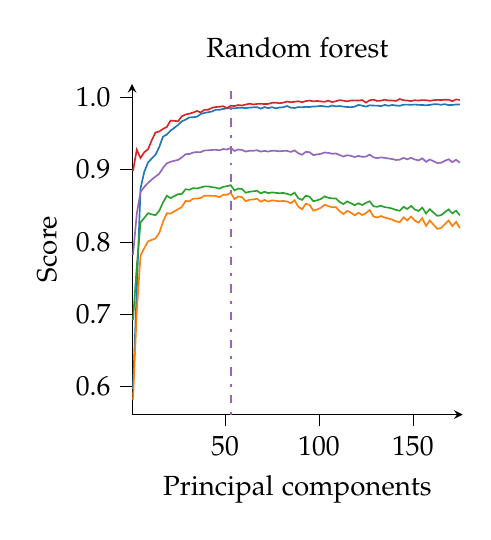
\begin{tikzpicture}

\definecolor{color0}{rgb}{0.12156862745098,0.466666666666667,0.705882352941177}
\definecolor{color1}{rgb}{1,0.498039215686275,0.0549019607843137}
\definecolor{color2}{rgb}{0.172549019607843,0.627450980392157,0.172549019607843}
\definecolor{color3}{rgb}{0.83921568627451,0.152941176470588,0.156862745098039}
\definecolor{color4}{rgb}{0.580392156862745,0.403921568627451,0.741176470588235}

\begin{axis}[
height=2.275590092707901in,
tick align=outside,
tick pos=left,
title={Random forest},
width=2.275590092707901in,
x grid style={white!69.0196078431373!black},
xlabel={Principal components},
xmin=0.5, xmax=176.5,
xtick style={color=black},
xtick={0,50,100,150,200},
xticklabels={
  \(\displaystyle {0}\),
  \(\displaystyle {50}\),
  \(\displaystyle {100}\),
  \(\displaystyle {150}\),
  \(\displaystyle {200}\)
},
y grid style={white!69.0196078431373!black},
ylabel={Score},
ymin=0.561477496219318, ymax=1.01863347578979,
ytick style={color=black},
ytick={0.5,0.6,0.7,0.8,0.9,1,1.1},
yticklabels={
  \(\displaystyle {0.5}\),
  \(\displaystyle {0.6}\),
  \(\displaystyle {0.7}\),
  \(\displaystyle {0.8}\),
  \(\displaystyle {0.9}\),
  \(\displaystyle {1.0}\),
  \(\displaystyle {1.1}\)
}
]
\addplot [semithick, color0]
table {%
1 0.59722126125097
3 0.734835181637817
5 0.874130828532667
7 0.897255518443422
9 0.910021818468807
11 0.915599575494005
13 0.920733589922345
15 0.9317329485511
17 0.94588067007524
19 0.948656264308016
21 0.954161909191095
23 0.957986929412309
25 0.962013094984398
27 0.966959458360583
29 0.969353278765588
31 0.972295923206796
33 0.97267159231806
35 0.973207693492041
37 0.977008734669172
39 0.97854605353126
41 0.979517697583872
43 0.980570103939348
45 0.982802055768921
47 0.982847704985427
49 0.984108576177909
51 0.984938801507521
53 0.985307317730692
55 0.984796479902308
57 0.985800164675294
59 0.985817527419282
61 0.985150498386723
63 0.985909698953989
65 0.986274224443756
67 0.986538408582648
69 0.984499040629036
71 0.986611235791801
73 0.985339245595103
75 0.986502003825798
77 0.984878208048563
79 0.986051587695095
81 0.986408148966353
83 0.988097139827444
85 0.985804161674806
87 0.985441912705817
89 0.986660549914611
91 0.986482487738967
93 0.986882007193021
95 0.986823869389597
97 0.987423889462149
99 0.987607258658971
101 0.988276340263476
103 0.987496515129508
105 0.987113350710469
107 0.988770218431461
109 0.987631648902874
111 0.988077422198818
113 0.987341059102131
115 0.986733981749148
117 0.986533380359752
119 0.987206529954149
121 0.989650996915168
123 0.988594511140455
125 0.987270045769131
127 0.989113484948624
129 0.988729947226513
131 0.98862031217692
133 0.987940545539679
135 0.989623848703039
137 0.988460788159652
139 0.989561008503821
141 0.988799482832435
143 0.988419811558422
145 0.989945382173628
147 0.990035773668564
149 0.989875111390907
151 0.990120988693737
153 0.989721267697889
155 0.989516497547703
157 0.989201760254715
159 0.989627916692931
161 0.990549096933001
163 0.990548794620309
165 0.989875615245394
167 0.990708419408475
169 0.989361918677886
171 0.989630876202953
173 0.990188710423507
175 0.990348969617574
};
\addplot [semithick, color1]
table {%
1 0.582257313472522
3 0.703576908020954
5 0.781639726424518
7 0.791747155948734
9 0.800985273344671
11 0.803008499378657
13 0.805048287937456
15 0.812919290986005
17 0.82813933496932
19 0.839933116555785
21 0.839309142048382
23 0.842509138263084
25 0.845439741288737
27 0.848610054766798
29 0.85678946496199
31 0.856277009947024
33 0.859955337639341
35 0.860123259455397
37 0.860938364271219
39 0.863959723045448
41 0.864232333737714
43 0.863886222254228
45 0.863757780633677
47 0.86197592088912
49 0.865409748803938
51 0.865321722162827
53 0.868231867499802
55 0.859592104145547
57 0.86297595089453
59 0.862128074631303
61 0.856429656701178
63 0.858556111963573
65 0.858861994501162
67 0.859977785379148
69 0.855774022793033
71 0.858280168824287
73 0.856032169954336
75 0.857700992855943
77 0.857078007142211
79 0.856340272892281
81 0.856909088223292
83 0.856077432884822
85 0.853622298820649
87 0.857868162690257
89 0.848907689971176
91 0.845332401780752
93 0.852978389180326
95 0.85137425932799
97 0.843434507421954
99 0.845169414238998
101 0.847376905343548
103 0.851579552651647
105 0.849655554970835
107 0.848125752212553
109 0.848365062438951
111 0.842686412534691
113 0.838695782531866
115 0.843074147061593
117 0.840605276059006
119 0.836932097295082
121 0.840583884048016
123 0.837312703921384
125 0.840018805083009
127 0.844207255677485
129 0.83544900742103
131 0.833865847195833
133 0.836018819854903
135 0.833836560068985
137 0.832537864981194
139 0.831074075048609
141 0.828459007070198
143 0.82766717675864
145 0.834147079596506
147 0.830003602957333
149 0.83537769010043
151 0.829650792881424
153 0.826785447468374
155 0.83298837959706
157 0.822308450539082
159 0.829821525050363
161 0.823918158627986
163 0.818280026644804
165 0.819538563876441
167 0.824830290323117
169 0.829722329933951
171 0.822160585724072
173 0.827917295395416
175 0.819251633217559
};
\addplot [semithick, color2]
table {%
1 0.692467628538399
3 0.766586579272089
5 0.82724677813506
7 0.833419252740925
9 0.839880037128331
11 0.838178996076448
13 0.837216511296203
15 0.843361051374326
17 0.854912213512556
19 0.864066067904858
21 0.860791910450187
23 0.863559885719853
25 0.866150919723699
27 0.866638036819272
29 0.872951999889314
31 0.872298423253009
33 0.874606549787485
35 0.87414080057987
37 0.875385333746744
39 0.876877302194397
41 0.877004526400047
43 0.875881832997461
45 0.875249715545295
47 0.873762509241852
49 0.876387752799132
51 0.877239605645773
53 0.878699686918563
55 0.871448023788113
57 0.874024029005874
59 0.873254174985233
61 0.868305261931905
63 0.869520154629273
65 0.87010253722489
67 0.870959811344763
69 0.867431710746304
71 0.869549539380749
73 0.8676637127434
75 0.868593988059667
77 0.868018836741884
79 0.867541987853898
81 0.867897136839601
83 0.866736389213694
85 0.865044755497167
87 0.868266837595929
89 0.860656485035825
91 0.85826774185107
93 0.864111532940603
95 0.862574607759479
97 0.85645265492087
99 0.857756215209664
101 0.859559874014496
103 0.863124954158872
105 0.861198961396998
107 0.860384406268404
109 0.860250743224491
111 0.855405719700441
113 0.852450048249788
115 0.856210690732954
117 0.853756517918072
119 0.85092815014534
121 0.853629080319015
123 0.851107090716629
125 0.854183268387832
127 0.856424770547738
129 0.849550808090464
131 0.848749447038843
133 0.850227306881538
135 0.848201146373335
137 0.847570784823426
139 0.846266670716523
141 0.844449561537903
143 0.84322225694787
145 0.848684919786359
147 0.845706920310201
149 0.849950255477111
151 0.845009534669244
153 0.842963522910178
155 0.847607984438977
157 0.839378965326265
159 0.845470319646793
161 0.840701996211717
163 0.836252514189232
165 0.8371611474015
167 0.841203939044478
169 0.845062320986516
171 0.839640601411967
173 0.843389740830659
175 0.836905417068356
};
\addplot [semithick, color3]
table {%
1 0.898439980870397
3 0.927752271640363
5 0.91622668579627
7 0.924234337637494
9 0.928334768053563
11 0.941023433763749
13 0.951573409851746
15 0.952936394069823
17 0.956452415112386
19 0.959184122429459
21 0.96797800095648
23 0.967585844093735
25 0.967002391200382
27 0.97403156384505
29 0.97637494021999
31 0.977547584887614
33 0.979109516977523
35 0.98125681492109
37 0.979302725968436
39 0.982819703491153
41 0.98301099952176
43 0.985552367288379
45 0.986724055475849
47 0.987111429937829
49 0.987894787183166
51 0.985164036346246
53 0.988481109516978
55 0.988087039693926
57 0.989455762792922
59 0.988873266379723
61 0.99004399808704
63 0.991410808225729
65 0.990240076518412
67 0.99102056432329
69 0.991216642754663
71 0.990823529411765
73 0.991018651362984
75 0.992583452893352
77 0.992775705404113
79 0.991995217599235
81 0.992775705404113
83 0.994339550454328
85 0.993361071257772
87 0.993947393591583
89 0.994729794356767
91 0.993361071257772
93 0.994923959827834
95 0.995705404112865
97 0.994529890004782
99 0.995120038259206
101 0.994531802965088
103 0.993947393591583
105 0.995511238641798
107 0.993555236728838
109 0.994728837876614
111 0.99628981348637
113 0.995509325681492
115 0.994529890004783
117 0.995705404112865
119 0.995897656623625
121 0.995704447632712
123 0.996288857006217
125 0.992775705404113
127 0.996094691535151
129 0.996876135820182
131 0.995119081779053
133 0.995509325681492
135 0.996875179340029
137 0.995706360593018
139 0.995703491152559
141 0.995116212338594
143 0.997853658536585
145 0.996096604495457
147 0.995705404112865
149 0.994922046867528
151 0.996093735054998
153 0.995707317073171
155 0.996288857006217
157 0.996093735054998
159 0.995312290769967
161 0.996095648015304
163 0.996679100908656
165 0.996290769966523
167 0.996874222859876
169 0.996877092300335
171 0.994729794356767
173 0.997266379722621
175 0.996485891917743
};
\addplot [semithick, color4]
table {%
1 0.782025546315744
3 0.839332247617965
5 0.869291935346631
7 0.876287400220564
9 0.881719876917005
11 0.886501926773996
13 0.890577135428357
15 0.894586157109603
17 0.902626078302082
19 0.908867412969607
21 0.911002534404812
23 0.912394537250977
25 0.913612386603002
27 0.917040810214638
29 0.921586353886293
31 0.921705495448873
33 0.923772637002286
35 0.924449559173957
37 0.924289330167027
39 0.926683900222187
41 0.926844121101328
43 0.927359835976764
45 0.927568469597156
47 0.926875116709293
49 0.928703109996736
51 0.927933185821485
53 0.930214957378713
55 0.926006778155564
57 0.928012997548613
59 0.927376114883806
61 0.92505556803743
63 0.926382421098627
65 0.926204578071884
67 0.926989985329128
69 0.925068082063457
71 0.926112556533024
73 0.925128308662709
75 0.926344151086026
77 0.926095765530172
79 0.925497361846843
81 0.92602164468961
83 0.926029111458864
85 0.924638849009363
87 0.926747444962935
89 0.922747050628139
91 0.920766326401275
93 0.924751337037949
95 0.924223368507371
97 0.920207031657441
99 0.921186911768155
101 0.922017175008161
103 0.923808885050341
105 0.923354696176
107 0.922086887457966
109 0.922505484193032
111 0.920345544368648
113 0.918296695412141
115 0.920054066064396
117 0.919172401537812
119 0.917575764396796
121 0.919145554126255
123 0.917847932366789
125 0.918159729815988
127 0.920913893838103
129 0.917180350349977
131 0.915962953034149
133 0.91702598913301
135 0.916408115220916
137 0.91552476265976
139 0.914818228398054
141 0.913480200908371
143 0.913886301691896
145 0.916357916108921
147 0.91441617452562
149 0.916602373470742
151 0.914255102082737
153 0.912864332511622
155 0.915842851809721
157 0.910929272358059
159 0.914153585265048
161 0.911684877045454
163 0.90930579712454
165 0.90971518910248
167 0.91232063655394
169 0.914544531236055
171 0.910499991285467
173 0.913785507062653
175 0.909653264887392
};
\addplot [semithick, color4, dash pattern=on 1pt off 3pt on 3pt off 3pt]
table {%
53 0.561477496219318
53 1.01863347578979
};
\end{axis}

\end{tikzpicture}

    \caption{}
    \label{fig:q1-RF}
  \end{subfigure}%
   \hfill
  \begin{subfigure}[b]{0.5\textwidth}
    % This file was created by tikzplotlib v0.9.8.
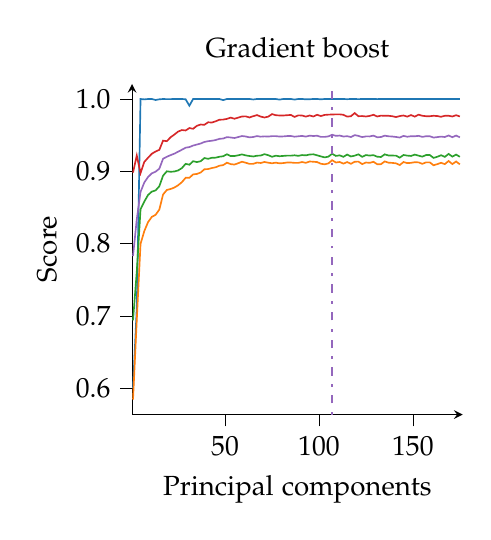
\begin{tikzpicture}

\definecolor{color0}{rgb}{0.12156862745098,0.466666666666667,0.705882352941177}
\definecolor{color1}{rgb}{1,0.498039215686275,0.0549019607843137}
\definecolor{color2}{rgb}{0.172549019607843,0.627450980392157,0.172549019607843}
\definecolor{color3}{rgb}{0.83921568627451,0.152941176470588,0.156862745098039}
\definecolor{color4}{rgb}{0.580392156862745,0.403921568627451,0.741176470588235}

\begin{axis}[
height=2.275590092707901in,
tick align=outside,
tick pos=left,
title={Gradient boost},
width=2.275590092707901in,
x grid style={white!69.0196078431373!black},
xlabel={Principal components},
xmin=0.5, xmax=176.5,
xtick style={color=black},
xtick={0,50,100,150,200},
xticklabels={
  \(\displaystyle {0}\),
  \(\displaystyle {50}\),
  \(\displaystyle {100}\),
  \(\displaystyle {150}\),
  \(\displaystyle {200}\)
},
y grid style={white!69.0196078431373!black},
ylabel={Score},
ymin=0.563723319050758, ymax=1.0207750800452,
ytick style={color=black},
ytick={0.5,0.6,0.7,0.8,0.9,1,1.1},
yticklabels={
  \(\displaystyle {0.5}\),
  \(\displaystyle {0.6}\),
  \(\displaystyle {0.7}\),
  \(\displaystyle {0.8}\),
  \(\displaystyle {0.9}\),
  \(\displaystyle {1.0}\),
  \(\displaystyle {1.1}\)
}
]
\addplot [semithick, color0]
table {%
1 0.600477159352101
3 0.711110568369543
5 0.999955056179775
7 0.999436657216473
9 0.999955156950673
11 0.99997557997558
13 0.99859295910538
15 0.999547270194522
17 0.999955156950673
19 0.999751163187149
21 0.999820627802691
23 0.999930736926253
25 1
27 1
29 0.99955106565224
31 0.990702463238936
33 0.999955156950673
35 0.999910213130448
37 1
39 1
41 1
43 1
45 1
47 0.99997557997558
49 0.998400695237564
51 1
53 1
55 1
57 1
59 1
61 1
63 1
65 0.999302027297593
67 1
69 1
71 0.999955056179775
73 1
75 1
77 0.999955156950673
79 0.999118587110392
81 1
83 1
85 1
87 0.999180460810498
89 1
91 1
93 0.999522779179722
95 0.999612435497859
97 1
99 1
101 0.999506021061118
103 0.999955156950673
105 1
107 1
109 1
111 1
113 1
115 0.999685796342016
117 1
119 1
121 0.999730639391344
123 1
125 1
127 1
129 1
131 0.999820627802691
133 1
135 0.999885793106028
137 1
139 0.999840950056701
141 1
143 1
145 1
147 1
149 1
151 0.999885893876925
153 1
155 1
157 1
159 1
161 1
163 1
165 0.999930636155355
167 1
169 1
171 1
173 1
175 1
};
\addplot [semithick, color1]
table {%
1 0.58449839909596
3 0.694545214460207
5 0.799704305914851
7 0.817293705880506
9 0.829745083267321
11 0.836988816752805
13 0.839783400637776
15 0.847081040919993
17 0.867955878659968
19 0.87421590969941
21 0.875514523541783
23 0.877555405682378
25 0.880676745253144
27 0.884983984958519
29 0.890982781510758
31 0.891022261706265
33 0.895745377320341
35 0.896358977341761
37 0.898318063349268
39 0.902797191124307
41 0.903117281916062
43 0.904540738114626
45 0.905586575302501
47 0.907738566092224
49 0.908567282746981
51 0.91192849202964
53 0.909919309912495
55 0.909325437294232
57 0.911186353908735
59 0.913224885471657
61 0.911877483293911
63 0.910213921033146
65 0.910360161863031
67 0.91205585530191
69 0.91150378991412
71 0.912902971274205
73 0.911880237790568
75 0.911111377774577
77 0.911948511639329
79 0.911031190393099
81 0.911395116319435
83 0.912138822569239
85 0.912144894279399
87 0.91167355036939
89 0.911657552407911
91 0.912826427011147
93 0.911680752591083
95 0.913541495174207
97 0.91322749455748
99 0.912787343810299
101 0.910457244598565
103 0.909633633018138
105 0.910902922803927
107 0.915318068888729
109 0.91217029962941
111 0.912890846318752
113 0.910626007950972
115 0.912759746680478
117 0.910370640675519
119 0.913238963548504
121 0.913389789205069
123 0.909929878279591
125 0.912156848434825
127 0.911657930937701
129 0.913138703932463
131 0.90980067959946
133 0.909867679372342
135 0.9137020813599
137 0.911931498110121
139 0.911617423172301
141 0.911033361861554
143 0.908660443082968
145 0.912837036000953
147 0.911325696725625
149 0.911690842718102
151 0.912595479985006
153 0.912347581748586
155 0.910307789496814
157 0.912343926628001
159 0.912347318162598
161 0.908332720761343
163 0.909919443321165
165 0.911761589012665
167 0.909944211633236
169 0.914256144184767
171 0.910004817022392
173 0.913569959229572
175 0.909633499609468
};
\addplot [semithick, color2]
table {%
1 0.693860588186648
3 0.761266907042525
5 0.847455095699409
7 0.85814946521674
9 0.867229193164921
11 0.871921851038143
13 0.87356458037904
15 0.879345480751021
17 0.893994513647079
19 0.899994454851895
21 0.899328703878698
23 0.899769718339221
25 0.901187798173528
27 0.904422880313242
29 0.910321387822326
31 0.909102861779526
33 0.913910478201278
35 0.912801457246958
37 0.913906080084742
39 0.91831076901138
41 0.917270990829357
43 0.918717072704449
45 0.918862153030851
47 0.920150359004712
49 0.920826270156352
51 0.923535568481933
53 0.921094120415459
55 0.921094507594081
57 0.922126932361603
59 0.923366723230051
61 0.921984531049316
63 0.921162261639504
65 0.920528825005478
67 0.921511506795139
69 0.921843162444666
71 0.923695402292872
73 0.922270995983839
75 0.92008912795755
77 0.92155024870831
79 0.920874046601856
81 0.921262338687648
83 0.921715185188628
85 0.921615133321455
87 0.922134809238973
89 0.92134077392626
91 0.92246364832241
93 0.922053878068597
95 0.923167974403954
97 0.923518774036849
99 0.922111809296067
101 0.92061188203032
103 0.919228917709697
105 0.920279805673989
107 0.924237835907056
109 0.921270649184521
111 0.922065650645469
113 0.920006191574565
115 0.923159988871448
117 0.920544326508925
119 0.921627575969626
121 0.923464786780374
123 0.920025421906584
125 0.922433889259609
127 0.921731268679298
129 0.92238658052776
131 0.920172596238642
133 0.919786576046323
135 0.923474404940506
137 0.921846027100073
139 0.921759437658457
141 0.921703291886696
143 0.918885209818666
145 0.922561460131922
147 0.921714156462307
149 0.921222809281307
151 0.923095589857119
153 0.921659872996399
155 0.920271658901523
157 0.922468143997433
159 0.922483932059776
161 0.918517504107247
163 0.920081759419155
165 0.922239589931981
167 0.919959655128522
169 0.924036637118789
171 0.920339401735935
173 0.923106757820066
175 0.920049529657888
};
\addplot [semithick, color3]
table {%
1 0.898243902439024
3 0.92189287422286
5 0.897474892395983
7 0.912888570062171
9 0.918756575801052
11 0.924228598756576
13 0.927346724055476
15 0.929692969870875
17 0.942395026303204
19 0.941610712577714
21 0.947077953132472
23 0.950792922046867
25 0.954889526542324
27 0.957036824485892
29 0.956457197513152
31 0.959776183644189
33 0.958797704447633
35 0.962898134863701
37 0.964663797226207
39 0.964268770923003
41 0.967788617886179
43 0.967395504543281
45 0.969152558584409
47 0.97130081300813
49 0.971500717360115
51 0.972473457675753
53 0.974230511716882
55 0.972669536107126
57 0.974232424677188
59 0.975793400286944
61 0.975984696317551
63 0.974430416068866
65 0.976183644189383
67 0.977747489239598
69 0.975594452415112
71 0.974425633668101
73 0.975594452415112
75 0.979111429937829
77 0.977545671927308
79 0.97716212338594
81 0.977156384505022
83 0.977546628407461
85 0.977941654710665
87 0.975200382592061
89 0.977356288857006
91 0.977155428024869
93 0.975594452415112
95 0.977160210425634
97 0.97578574844572
99 0.978135820181731
101 0.97637780966045
103 0.977941654710665
105 0.978330942132951
107 0.978522238163558
109 0.978716403634624
111 0.978719273075084
113 0.978131037780966
115 0.975593495934959
117 0.976178861788618
119 0.980477283596366
121 0.976177905308465
123 0.976381635581062
125 0.975790530846485
127 0.976571975131516
129 0.978133907221425
131 0.975788617886179
133 0.976965088474414
135 0.976767097082735
137 0.976765184122429
139 0.976178861788618
141 0.975004304160689
143 0.97637494021999
145 0.977157340985175
147 0.975595408895265
149 0.977744619799139
151 0.975596365375418
153 0.978330942132951
155 0.976764227642277
157 0.976180774748924
159 0.976177905308465
161 0.976765184122429
163 0.976376853180296
165 0.975402199904352
167 0.976764227642276
169 0.976765184122429
171 0.975791487326638
173 0.977548541367767
175 0.97579531324725
};
\addplot [semithick, color4]
table {%
1 0.782814458841815
3 0.833681366927328
5 0.871544812840382
7 0.88450524740946
9 0.892136285245678
11 0.897165488911998
13 0.899451483943924
15 0.903620984971089
17 0.917365643926025
19 0.920107702385579
21 0.922347081752579
23 0.924389348803215
25 0.927080602417497
27 0.929807469319265
29 0.932613493254474
31 0.933521019702505
33 0.935603914601139
35 0.937010498439717
37 0.938423846824096
39 0.94055964720593
41 0.941667449330237
43 0.942267663904974
45 0.943211215775535
47 0.944889842004273
49 0.945333184800393
51 0.947267248973245
53 0.946758373573768
55 0.946032466678366
57 0.947355107355928
59 0.948768797168942
61 0.948145419707285
63 0.946914960835368
65 0.947440916336466
67 0.948693038310257
69 0.947868060499603
71 0.948281420649866
73 0.948058018304228
75 0.948585225184111
77 0.94861242744043
79 0.948046236921776
81 0.948247306927201
83 0.948703755044584
85 0.948819342634485
87 0.947843872197372
89 0.948419812367761
91 0.948944029283571
93 0.947963007748127
95 0.949300156927316
97 0.94880998103799
99 0.949170474200889
101 0.947569541012488
103 0.947559436386842
105 0.948299653148213
107 0.950527052330008
109 0.949029706332622
111 0.949406004576716
113 0.948102182263478
115 0.948521358788244
117 0.947438892523974
119 0.950020805562714
121 0.948995352090537
123 0.947285202555973
125 0.948259187837254
127 0.948223745737047
129 0.949347744888069
131 0.947072573697636
133 0.947395993700139
135 0.949271337385419
137 0.948404680429431
139 0.948084961482875
141 0.947492531525012
143 0.946669227773229
145 0.948963586406717
147 0.947788706866025
149 0.948530731597907
151 0.948439719414634
153 0.949032460589269
155 0.9475778648495
157 0.948468721343133
159 0.948462731376665
161 0.946621917894398
163 0.947300585071087
165 0.947956594528722
167 0.947396326704495
169 0.949552398946318
171 0.947157261945506
173 0.949445988549005
175 0.946981629259943
};
\addplot [semithick, color4, dash pattern=on 1pt off 3pt on 3pt off 3pt]
table {%
107 0.563723319050758
107 1.0207750800452
};
\end{axis}

\end{tikzpicture}

    \caption{}
    \label{fig:q1-GB}
  \end{subfigure}
  \caption{{Four figures displaying hyperparameter search for the Ferrenti approach. The best estimator is visualized for all hyperparameters as a function of principal components during a grid search with a $5\times5$ stratified cross-validation, and the dotted lines mark the optimal hyperparameter-combination. Train stands for normal training accuracy, while test is the balanced accuracy on the test set. Precision, recall, and F1 scores are based on the test set. The number of principal components that explain the $95\%$ accumulated variance is $144$, while the optimal model is found using the F1-score.}}
  \label{fig:01-pca}
\end{figure}

\clearpage

\section*{Supplementary results}
Table~\ref{tab:03-probability-candidates} displays the 66 predicted candidates that all four machine learning models, using the data set derived in the intuitive approach, agreed on with a cut-off set to $0.75$. All band gaps are taken from the Materials Project database as calculated using DFT and the PBE functional. Note that materials can appear several times  on  the  list due  to  different  structures of the same composition. The  list  contains $5$ elementary (unary), $46$  binary and  $15$ ternary compounds. 

\begin{center}
\begin{longtable}{M{3.5cm} M{6.5cm} M{2.0cm}}
\caption{The $66$ predicted candidates that all models in the intuitive approach agreed on to a cut-off of $0.75$. All band gaps were taken from the Materials Project (MP) database, and materials can appear several times in the list due to different structures. The list contains $5$ elementary (unary), $46$ binary and $15$ ternary compounds.}
\label{tab:03-probability-candidates}  
\\ \hline
Compound formula & MP ID & Band gap from MP (eV) \\
\hline
  Ge & mp-137 & 0.87\\
  CdTe & mp-406 & 1.22\\
  HgSe & mp-820 & 0.12\\
  GeTe & mp-938 & 0.82\\
  MgTe & mp-1039 & 2.36\\
  CdSe & mp-1070 & 0.55\\
  GaSb & mp-1156 & 0.36\\
  BP & mp-1479 & 1.46\\
  MoSe$_2$ & mp-1634 & 1.41\\
  BN & mp-1639 & 4.64\\
  YbTe & mp-1779 & 1.52\\
  SnS & mp-1876 & 0.95\\
  SnTe & mp-1883 & 0.66\\
  GeTe & mp-2612 & 0.61\\
  AlSb & mp-2624 & 1.26\\
  CdSe & mp-2691 & 0.50\\
  SnSe & mp-2693 & 0.82\\
  CdSnAs$_2$ & mp-3829 & 0.30\\
  GaCuTe$_2$ & mp-3839 & 0.55\\
  ZnGeAs$_2$ & mp-4008 & 0.56\\
  ZnGeP$_2$ & mp-4524 & 1.20\\
  GaAgTe$_2$ & mp-4899 & 0.19\\
  CdSnP$_2$ & mp-5213 & 0.67\\
  GaCuS$_2$ & mp-5238 & 0.70\\
  SnS & mp-10013 & 0.23\\
  BAs & mp-10044 & 1.25\\
  GeSe & mp-10759 & 0.44\\
  MgSe & mp-10760 & 1.97\\
  CdTe & mp-12779 & 0.61\\
  MgSe & mp-13031 & 2.54\\
  MgTe & mp-13033 & 2.31\\
  TePb & mp-19717 & 1.05\\
  InAs & mp-20305 & 0.30\\
  InP & mp-20351 & 0.46\\
  InAgSe$_2$ & mp-20554 & 0.36\\
  InN & mp-22205 & 0.47\\
  AgI & mp-22894 & 1.39\\
  CuI & mp-22895 & 1.17\\
  CuBr & mp-22913 & 0.48\\
  CuCl & mp-22914 & 0.80\\
  AgI & mp-22919 & 1.00\\
  AgI & mp-22925 & 1.72\\
  Br & mp-23154 & 1.32\\
  TlI & mp-23197 & 2.25\\
  AgBr & mp-23231 & 0.79\\
  BC$_2$N & mp-30148 & 2.10\\
  CuI & mp-569346 & 1.21\\
  Hg & mp-569360 & 0.22\\
  Ga$_2$Os & mp-570875 & 0.66\\
  BC$_2$N & mp-629458 & 1.84\\
  InP & mp-966800 & 0.51\\
  GeC & mp-1002164 & 1.84\\
  TlP & mp-1007776 & 0.12\\
  BC$_2$N & mp-1008523 & 1.64\\
  BP & mp-1008559 & 1.07\\
  OsC & mp-1009540 & 0.17\\
  SiSn & mp-1009813 & 0.41\\
  ZnCdSe$_2$ & mp-1017534 & 1.85\\
  MgSe & mp-1018040 & 2.57\\
  AlSb & mp-1018100 & 0.91\\
  AlBi & mp-1018132 & 0.30\\
  Ge & mp-1067619 & 0.791\\
  Ga$_2$Ru & mp-1072429 & 0.12\\
  ZnCd$_3$Se$_4$ & mp-1078597 & 1.72\\
  BC$_2$N & mp-1079201 & 1.17\\
  Ge & mp-1198022 & 0.67\\
  \hline
\end{longtable}
\end{center}


Table~\ref{tab:04-probability-candidates} displays the $47$ predicted candidates that all four machine learning models and all three approaches agreed upon. The list contains $8$ elemental, $29$ binary, and $10$ tertiary compounds.

\begin{center}
\begin{longtable}{M{3.5cm} M{6.5cm} M{2.0cm}}
\caption{A table displaying the $46$? predicted candidates that all models and all approaches agree on.}
\label{tab:03-probability-candidates}  
\hline
Compound formula & MP ID & Band gap from MP (eV) \\
\hline
  P & mp-157 & 7.47\\
  SiRu & mp-189 & 0.63\\
  BN & mp-344 & 0.41\\
  HgSe & mp-820 & 3.96\\
  FeSi & mp-871 & 2.06\\
  MgTe & mp-1039 & 6.62\\
  CdSe & mp-1070 & 3.91\\
  BP & mp-1479 & 2.89\\
  CdSe & mp-2691 & 2.40\\
  ZnSiAs$_2$ & mp-3595 & 1.57\\
  ZnGeAs$_2$ & mp-4008 & 1.52\\
  CdSnP$_2$ & mp-5213 & 0.95\\
  Si$_2$Mo & mp-8938 & 0.66\\
  BAs & mp-10044 & 0.61\\
  GeSe & mp-10759 & 1.26\\
  N$_2$ & mp-12103 & 0.50\\
  BeSiN$_2$ & mp-15704 & 0.82\\
  InP & mp-20351 & 0.30\\
  InN & mp-22205 & 0.55\\
  AgCl & mp-22922 & 0.56\\
  I & mp-23153 & 1.20\\
  Br & mp-23154 & 0.19\\
  TlI & mp-23197 & 0.67\\
  AgBr & mp-23231 & 0.70\\
  H$_2$ & mp-23907 & 0.23\\
  Ge$_3$As$_4$ & mp-569600 & 1.25\\
  TlCl & mp-569639 & 0.44\\
  Sn$_3$As$_4$ & mp-570377 & 1.97\\
  H$_2$ & mp-634659 & 0.61\\
  N$_2$ & mp-672234 & 2.54\\
  TiFe$_2$Ge & mp-866375 & 2.31\\
  InP & mp-966800 & 1.05\\
  GeC & mp-1002164 & 0.30\\
  B$_2$AsP & mp-1008528 & 0.46\\
  BP & mp-1008559 & 0.36\\
  BeSiAs$_2$ & mp-1009087 & 0.47\\
  OsC & mp-1009540 & 1.39\\
  ScP & mp-1009746 & 1.17\\
  SiSn & mp-1009813 & 0.48\\
  SnC & mp-1009820 & 0.80\\
  AlBi & mp-1018132 & 1.00\\
  Al$_3$BN$_4$ & mp-1019380 & 1.72\\
  GeRu & mp-1025397 & 1.32\\
  PbS & mp-1057015 & 2.25\\
  Ge & mp-1067619 & 0.79\\
  ZnCd$_3$S$_4$ & mp-1078780 & 2.10\\
  Ga$_4$BiAs$_3$ & mp-1079228 & 1.21\\
  \hline
\end{longtable}
\end{center}



\bibliography{apssamp}% Produces the bibliography via BibTeX.

\end{document}

